\documentclass{article}
\usepackage{graphicx,fancyhdr,amsmath,amssymb,amsthm,subfig,url,hyperref}
\usepackage[margin=1in]{geometry}
\usepackage{xltxtra}
\usepackage{xgreek}
\usepackage{amsfonts}
\usepackage{amssymb}
\usepackage{amsmath}
\usepackage{amsthm}
\usepackage{mathtools}

\usepackage{caption}
\usepackage{subfig}
\setmainfont[Mapping=tex-text]{Times New Roman}
%----------------------- Macros and Definitions --------------------------

%% FILL THIS OUT
\newcommand{\studentname}{Νικόλαος Ζαρίφης}
\newcommand{\suid}{03112178}
\newcommand{\exerciseset}{Exercise Set 3}
%% END



\renewcommand{\theenumi}{\bf \Alph{enumi}}

%\theoremstyle{plain}
%\newtheorem{theorem}{Theorem}
%\newtheorem{lemma}[theorem]{Lemma}

\fancypagestyle{plain}{}
\pagestyle{fancy}
\fancyhf{}
\fancyhead[RO,LE]{\bfseries\large NTUAthens}
\fancyhead[LO,RE]{\bfseries\large Θεωρία γράφων}
\fancyfoot[LO,RE]{\bfseries\large \studentname: nick.zarifis@hotmail.com}
\fancyfoot[RO,LE]{\bfseries\thepage}
\renewcommand{\headrulewidth}{1pt}
\renewcommand{\footrulewidth}{1pt}

\graphicspath{{figures/}}
\usepackage{tikz}
%-------------------------------- Title ----------------------------------

\title{Θεωρία γράφων \\ \exerciseset}
\author{\studentname \qquad  ID: \suid}

%--------------------------------- Text ----------------------------------
\DeclarePairedDelimiter\floor{\lfloor}{\rfloor}
\newtheorem{lemma}{Lemma}
\begin{document}
\maketitle
\section*{Άσκηση 1}
Παίρνουμε έναν κύκλο κι ένοουμε σε αυτόν μια κορυφή με μια ακμή σε 2 κορυφές. Σε κάθε σκελετικό δέντρο που διατηρή αποστάσεις η νεα κορυφή θα διατηρεί αποστάσεις κι η γειτονική της, γιατί σε κάθε σκελετικό η ακμή που τις ενώνει δεν φεύγει αλλίως δεν θα ήταν συνεκτικό και η extra κορυφή πρέπει πάντα να περάσει από την γειτόνικη τις για να παει σε μια οποιαδήποτε.
\section*{Άσκηση 2}
Το σκελέτικο δέντρο περιέχει ένα ύποσυνολο των ακμών, όποτε επιλέγοντας μια δυάδα (r,t),το μέγιστο σκελέτικο δέντρο ως προς τα φύλα είναι αυτό που έχει μια ρίζα κι όλες οι άλλες κορυφές είναι φύλλα, όποτε το γράφιμα μας θα έχει t+1 κορύφες κι η μια θα συνδέαιτε με όλες, τώρα μας μένει να δημιουργήσουμε από αυτό κι ένα με ελάχιστα φύλλα. Αυτό γίνεται ακολούθως: Στις κορυφές που είναι πριν τα φύλα βάζω ανα 2 ακμές ωστέ να δημιουργήσω κύκλους έτσι δημιουργώ δέντρο με -1 λειγότερα φύλλα, κάνοντας αυτή την διαδικάσια t-r φορές.
Παρακάτω έχουμε ένα σχήμα. 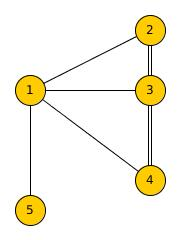
\includegraphics[height=100pt,width=100pt]{ex2} 
 \section*{Άσκηση 3}
Από την ανισότητα βλέπουμε πως το $d(u)=n-1,d(v)=1$ γιατί οι βάθμοι είναι μικρότεροι ή ίση του $n-1$, και το γραφημά μας είναι συνεκτίκο,επίσεις προκύπτει ότι οι κορυφές είναι γείτονες.Έστω ότι το n είναι περιττό τότε το $n-1$ είναι άρτιο όμως τότε πρεπει αν αφαιρέσουμε την κορυφή v να υπάρχει ένας κύκλος Euler από την κορυφή u όμως αυτό είναι άτοπο αφού η κορυφή θα έχει περριτό βαθμό. Άρα το n είναι άρτοιο.
\section*{Άσκηση 4}
Φτάνει να δείξουμε ότι υπάρχει μια κορύφη με περιττό βαθμό γιατί έτσι θα έχουμε 2 κόρυφες διαφορετικού parity έτσι για όποιοδηποτε n δεν θα έχουμε γράφημα Euler.Αν όλες έχουν άρτιο, τότε έστω $\forall u d(u)=2k,1\le k$ τότε $\sum_{u \in V(T)}d(u) \ge 2V(T) \rightarrow 2E(T)\ge 2V(T)$ όπου είναι άτοπο αφού σε κάθε δέντρο ισχυεί: $E=V-1$.
\section*{Άσκηση 5}
\begin{itemize} \item i
Αφού το n είναι περιττό  τότε θα πρέπει να μοιράσουμε στις κορυφές τους ζυγούς αριθμούς από το 1 ως το n που είναι $\frac{n -1} {2}$ όμως έχουμε n κορυφές και $n-1$ φόλιες και μπορούμε να μοιράσουμε ώστε να δώσουμε το πολύ 2 φόρες τον ίδιο βαθμό άρα απο θεώρημα περιστερώνα θα έχουμε ότι τουλάχιστον 3 κορυφές θα έχουν τον ίδιο βαθμό.
\item ii
Επαγωγική κατασκευή, το$ K_3$ είανι η βάση, έστω ότι έχουμε το n ωστο. Πέρνουμε 2 νέες κορύφες κι προσθέτουμε ακμές ενώνοντας τες κι τις 2 στις ίδιες κορυφές για να μην χαθεί η αρτιοτητα, πρώτα στις 2 με μέγαλυερο βαθμό μετά στις 2 με μικρότερο(εκτώς από αυτές με βαθμό 2) κοκ κι σταμάταμε όταν φτάσει σε έναν βαθμό που δεν θα έχουμε , σίγουρα υπάρχει γιατί έχουμε κένη φολιά . έτσι θα έχουμε όλες τις κορυφές  απο τρις κορυφες 2 βαθμού. Αυτό είναι μοναδικό γιατί από την βάση βλέπουμε ότι υπάρχει μοναδικός τρόποσ να πάμε στο έπομενο βημα. 
\end{itemize} 
\section*{Άσκηση 6}
\begin{itemize} \item i
Αφού έχουμε k+1 μη γειτονικές κορυφές, για να υπάρχει hamiltonian cicle θα πρέπει να πηγαίνει απο αυτές τις k+1 στις άλλες k κι πάλι πίσω γιατί αλλιώς δεν θα μπορούμε να διασχήσουμε όλες τις k+1 κορυφές. Όμως αν ξεκινήσουμε από το σύνολο με τις k+1, κι διασχήσουμε τις κορυφές η τελευταία κορυφή θα είναι του σύνολου k+1 κι δεν θα είναι η αρχική όπωτε δεν μπορούμε να πάμε πάλι στην άρχικη χωρίς να περάσουμε από μια από τις άλλες ξανά. Αν ξέκινουσαμε από τις λειγότερες δεν θα φτάναμε πότε στην τελευταία κορυφή πριν το τέλος.
\item ii
Απλά πέρνουμε το $P_n $ και κάνουμε το ακούλουθο , στις μονές κορυφές δεν κάνουμε τίποτα εκτώς από την πρώτη που την συνδέουμε με την τελευταία, κι στις ζυγές βάζουμε μια ακμή με μια αλλή ζυγή τύχαια. Η πρώτη κορυφή έχει βαθμό 2 γιατί συνδέαιτε με την δεύτερη κι την τελευταία, κι η τελευταία 3 γιατί συνδέαιτε με την πρώτη του μονοπάτιου , την προηγούμενη κι μια τυχαία. Θα μπορούσα να το αποδείξω κι με επαγώγηκη απόδειξη ως προς το κ, αλλά θα ήαν πάλι η ίδια κατασκευή απλά με την νέα κορυφή.
\end{itemize}
\section*{Άσκηση 7}
Το γράφημα μας είναι συνεκτίκο γιατί μια κορυφή συνδαιέται με τουλάχιστον k/2 + 1 κορυφές του άλλου, όπωτε κάθε κόρυφη από το ίδιο σύνολο θα έχει κοινό γείτονα απο περιστερόνα.\\
Μπορούμε να φτιάξουμε εύκολα ένα hamiltonian γράφημα απλά φτιάχνουμε έναν κύκλο κι προσθέτουμε ακμές ώστε να ισχυεί η σχέση. Τώρα έστω ότι υπάρχει γράφημα που να ίσχυει η σχέση κι δεν είναι hamiltonian, άρα μπορούμε να σχηματίσουμε ένα μεγιστότικο μη-hamiltonian
Παίρνοντας το μεγιστότικο μη-hamiltonian αυτό θα περιέχει ένα hamiltonian μονοπάτι, τα δυο άκρα του όμως δεν ενόνονται αλλιώς θα ήταν κύκλος, τώρα αφού είναι διμέρες κάθε κορύφη ενώνεται με μια κορυφή άλλου συνόλου, έτσι χωρίζουμε στο μονοπάτι της κορυφές σε όμαδες έτσι ώστε η (ν,ν+1) είναι στην ίδια όμαδα, έτσι έχουμε k/2 όμαδες. όμως και η δυο κορυφες έχουν βαθμό μεγαλύτερο του k/2 άρα απο περιστερόνα, έχουν ακμές σε ένα σύνολο έτσι πέρνοντας. Όμως αυτός είναι ένας hamiltonian κύκλος , άρα άτοπο η υπόθεση. Σχήμα είναι το ίδιο απο την απόδειξη του Θεωρήματος του Ore 7.3.
\section*{Άσκηση 8}
θα το δείξουμε χρησιμοποιώντας επάγωγη. Για n=4 έχουμε μόνο έναν δέντρο που έιναι διαφορό τις διμέρης κλίκας $K_{1,3}$.To $P_4$ όπου από προηγούμενη σειρά ασκήσεων έχουμε δείξει ότι το συμπλήρωμα του είναι ισομορφικό με το $P_4$ το όποιο είναι hamilton μόνοπατι.
Έστω ότι ισχυεί για κάθε δέντρο με n=k κορυφές. Όπωτε για να πάμε στις k+1 θα πρέπει να  προσθέσουμε μια κορυφή μαζί με μια ακμή και για κάθε κορυφή που έχει δημιουργούμε ένα νέο δέντρο έτσι. Προφανώς δεν εμφανίζεται η διμερής κλίκα που απαγορεύεται.Τώρα λοίπον πέρνωντας το συμπληρωμά του η κορυφή αφτή θα συνδέαιτε με όλες τις κόρυφες εκτώς από αυτή που συνδεόταν.Η νέα κορυφή θα συνδέαιτε με τουλάχιστον την μια από τις 2 κορυφές που είναι άκρα του μονοπατιού,όποτε θα έχουμε ένα μονοπάτι με k+1 κορυφές.\footnote{Μπόρει να σχημάτιστει κι κύκλος αλλα δεν επειρεάζει ότι θα ύπαρχει μονοπάτι}. Άρα απο Μ.Ε. ισχυεί. 
\end{document}
